
\section{Extra: The FAIMS approach in-depth}

\begin{sectionframe} % Custom environment required for section slides
	\frametitle{Extras: The FAIMS approach in-depth}
	%\framesubtitle{Subtitle}

% 	Some section slide content

% 	This is on another line
\end{sectionframe}


%----------------------------------------------------------------------------------------
\begin{frame}{Introduction to the FAIMS Project}
    \begin{itemize}
        \item The Field Acquired Information Management Systems (FAIMS) Project began in 2012 as a national Australian information infrastructure project in archaeology.
        \item Developed FAIMS Mobile for field data capture \parencite{Ballsun-Stanton2018-zd}.
        \item Use expanded beyond archaeology to geoscience, ecology, ethnography, linguistics, oral history.
        \item Has been customised for over 50 workflows at more than 30 projects. 
        \item Data and workflow modelling for customisations provided deep insights into field data capture and the infrastructure needed to support it.
    \end{itemize}
\end{frame}
%----------------------------------------------------------------------------------------
\begin{frame}{FAIMS Mobile software}
 \begin{figure}[H]
    \centering
    \vspace{-0.5cm}
        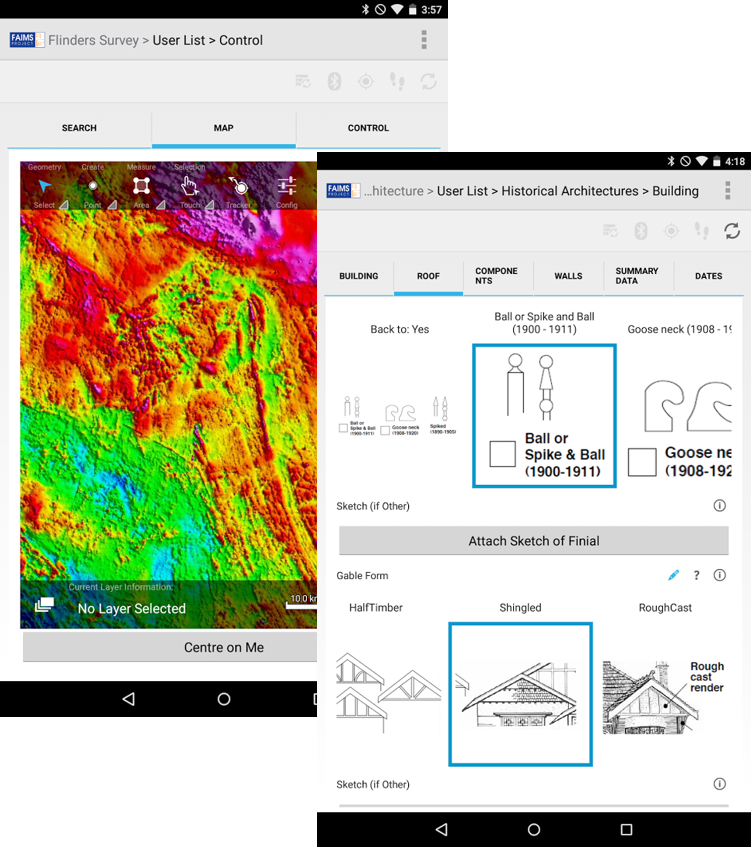
\includegraphics[height=.725\textheight]{figures/FAIMS-screenshots.png}
        \caption{FAIMS Mobile: GIS and `picture dictionaries'}
        \label{fig:figure10}
 \end{figure}
\end{frame}
%----------------------------------------------------------------------------------------
\begin{frame}{Field data capture infrastructure: a manifesto}
    \begin{itemize}
        \item Our domains deserve research-specific software.
        \item Diverse practices and limited resources require generalised software.
        \item Do one thing well with modular and federated software (but slice the pie thoughtfully).
        \item Open-source software supports open research and has other advantages (but is difficult to sustain). 
        \item Scope requirements carefully.
        \item Invest in outreach and engagement.
    \end{itemize}
\end{frame}
%----------------------------------------------------------------------------------------
\begin{frame}{Research specific}
    Field research needs (and deserves) research-specific software, contra \parencite{Roosevelt2015-kd}.
      \begin{itemize}
        \item Most commercial / mass-market software does not meet research needs.
        \item Risk of lock-in, unwelcome changes to features or business models, and product discontinuation.
    \end{itemize}
    \medskip{}
    Compare ecology: TERN, ALA, Biocollect, and associated research clouds \parencite{Tern2019-sp, Ala2019-by, Ala2019-cb}.
\end{frame}
%----------------------------------------------------------------------------------------
\begin{frame}{Generalised (not generic or bespoke)}
  Commercial software doesn't meet our needs, and bespoke development is too expensive and usually unsustainable.
      \begin{itemize}
        \item Generalised software can be deeply customised to accommodate our diverse data types, data models, workflows, etc.
        \item The code used to customise it describes the data model and workflow.
        \item Customisations can be published and re-deployed trivially.
        \item Can deliver research-grade software affordably.  
    \end{itemize}
    FAIMS Mobile cost perhaps 3x a single bespoke application, but has been customised 50x. Customisation cost is 1/10th bespoke, and still <1/2 even if `core' platform development costs are amortised across projects.
\end{frame}
%----------------------------------------------------------------------------------------
\begin{frame}{Generalised: customise using code}
 \begin{figure}[H]
    \centering
    \vspace{-0.5cm}
        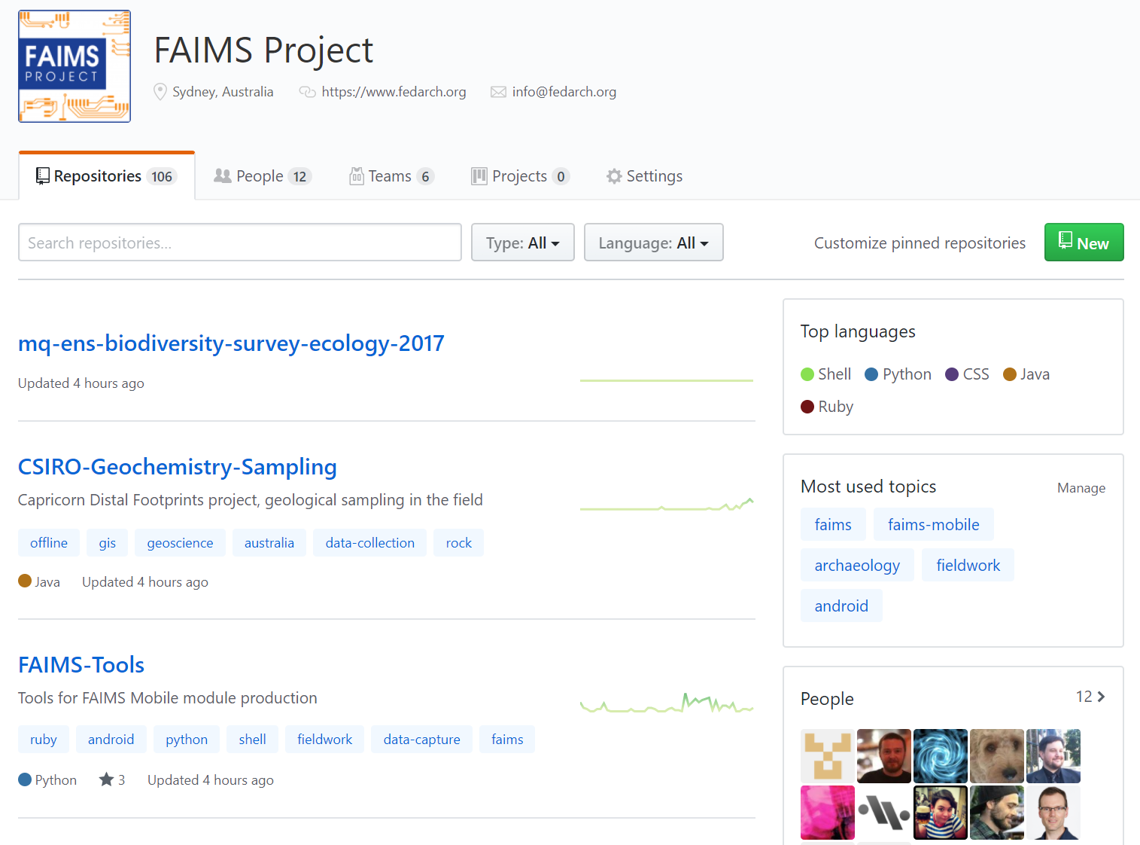
\includegraphics[height=.725\textheight]{figures/FAIMS-generalised.png}
        \caption{FAIMS Mobile customisations (XML files, mostly) on GitHub}
        \label{fig:figure11}
 \end{figure}
\end{frame}
%----------------------------------------------------------------------------------------
\begin{frame}{Modular and federated}
  \textbf{Do one thing well.}
      \begin{itemize}
        \item Identify other infrastructure in the domain and interoperate with it (via ETLs or APIs).
        \item It is better to divide by data-lifecycle phase rather than data type, since (1) our data is so integrated and (2) field data capture poses unique challenges.
    \end{itemize}
\end{frame}
%----------------------------------------------------------------------------------------
\begin{frame}{Modularise by data lifecycle phase}
 \begin{figure}[H]
    \centering
    \vspace{-0.5cm}
        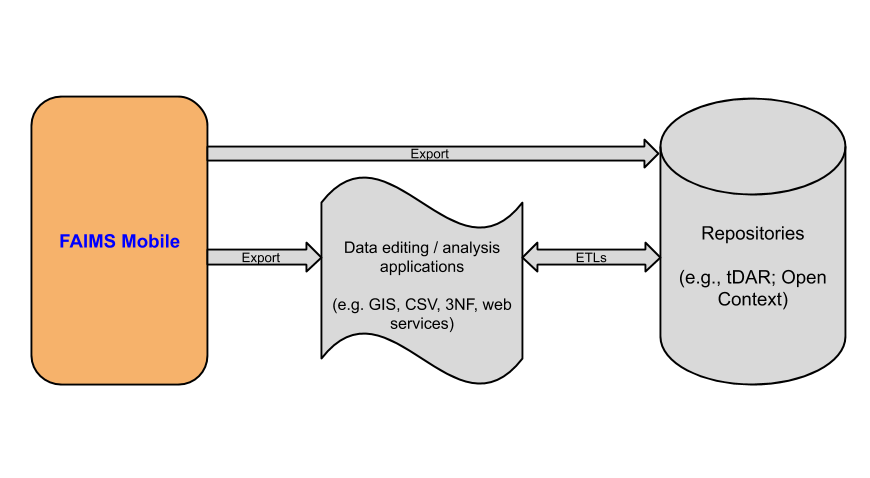
\includegraphics[height=.75\textheight]{figures/FAIMS-federation.png}
        \caption{FAIMS Mobile federation strategy}
        \label{fig:figure13}
 \end{figure}
\end{frame}
%----------------------------------------------------------------------------------------
\begin{frame}{Open source?}
  Open source has advantages but is difficult to sustain.
      \begin{itemize}
        \item Emerging open research principles strongly prefer OSS as opposed to proprietary ‘black boxes’.
        \item Transparency and reusability (esp. customisation code).
        \item Ability to hand off from one organisation to another (esp. `core' platform code).
        \item Ability to fork code prevents lock-in and mitigates unwelcome decisions by software developers.
        \item BUT OSS business models are hard to scale and rely on occasional injections of grant or institutional funding.
    \end{itemize}
\end{frame}
%----------------------------------------------------------------------------------------
\begin{frame}{Scope carefully}
  Talk to a wide range of potential users, seeking facts not opinions.
      \begin{itemize}
        \item Don’t ask researchers what they think, ask them what they have done - what software they have adopted and why, and what problems they have expended resources to solve. 
        \item ‘Lean startup’ methodology very useful, based around  testing of ideas through interviews with potential users \parencite{Strategyzer_AG2019-uu}.
        \item In our case, we over-invested in mobile GIS and under-invested in usability (especially a GUI for customisation).
    \end{itemize}
\end{frame}
%----------------------------------------------------------------------------------------
\begin{frame}{Spend on outreach and engagement}
  If you build it they will not come; people can't use technologies they don't know about.
      \begin{itemize}
        \item As per industry standards, dedicate at least 30\% of any information infrastructure budget to outreach and engagement (sales and marketing). 
        \item Typical academic outreach (journal articles, conference presentations, workshops, even booths at major conferences) are not enough.
    \end{itemize}
\end{frame}